\documentclass[a4paper]{article}

\usepackage{babel}
\usepackage[latin1]{inputenc}
\usepackage{amssymb}
\usepackage{framed}
\usepackage{graphicx} 
\usepackage{subcaption}


\setlength{\parindent}{0pt}
\setlength{\parskip}{3ex}

\begin{document}

\begin{center}
  {\large Artificial Neural Networks and Deep Architectures, DD2437}\\
  \vspace{7mm}
  {\huge Short report on lab assignment 1b\\[1ex]}
  {\Large Learning with backpropagation and generalisation in multi-layer perceptrons\\}
  \vspace{8mm}  
  {\Large Rakin Ali , Steinar Logi Geirsson and Hasan Alzubeidi}
  \vspace{4mm}
  {\large January 31 2024 }
\end{center}

\section{Main objectives and scope of the assignment}
The major objectives in this assignment was
\begin{itemize}
\item To gain a better theoretical foundation of Neural Networks learn by implementing Backpropagation algorithm and monitoring its parameters. 
\item Building Multilayered Perceptrons from scratch with plain Python programming using no imports and by using libraries used by the industry, in this case it was TensorFlow.
\item to observe how to improve generalization of a model and which parameters in the model has the most effects on generalization. 
\end{itemize}
The scope of this assignment are the instructions that were given excluding all non-mandatory tasks. The limitations was that all data were supervised and only one hidden layer was created. We did as the instructions and did not try different activation functions or making the MLP deeper. 
\section{Methods}
Most of the lab instructions were conducted twice in order to check if the results were reasonable but also so that each of us had gain a better theoretical foundation of the assignments. We discussed and had to ask ourselves \textit{is this result reasonable or is there a mistake in the code} and several times there were a few mistakes which were fixed. 


\section{Results and discussion}
\subsection{Classification and regression with a two-layer perceptron}
\textbf{Classification of linearly non-separable data:} For this assignment linearly non-separable data was generated. In the first part of the assignment the amount of hidden nodes was modified together with the learning rate. What was discovered was that as long as there were more than one hidden node, the model achieved good results however more nodes resulted in a more complex boundary. Below are figure \ref{fig:1Hidden} which contains one hidden neuron and figure \ref{fig:15Hidden} which contains 15 hidden neurons. This could be due to overfitting which is why a generalization check was conducted.

\begin{figure}[htb]
    \centering
    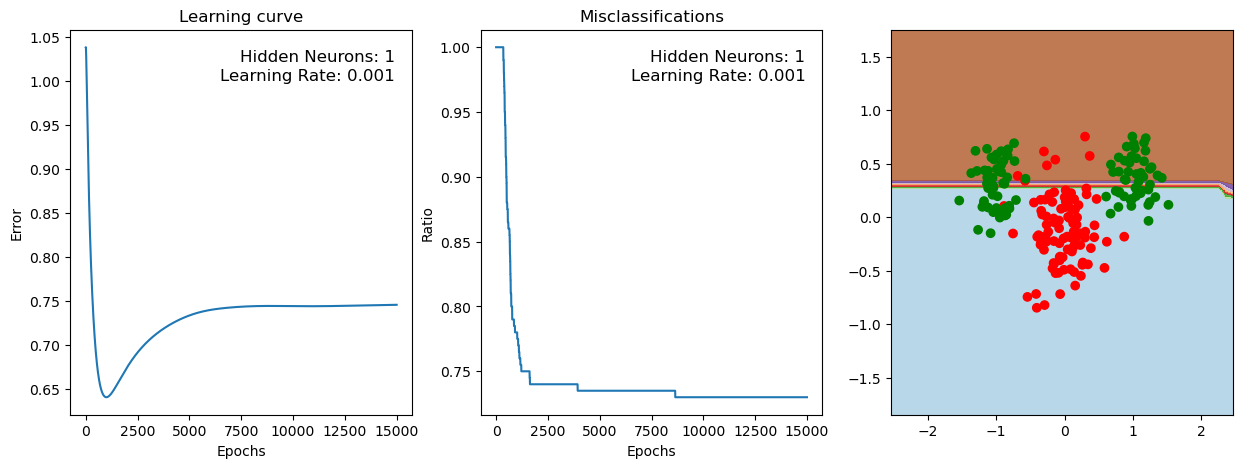
\includegraphics[width=10cm]{Labs/Lab 1/Lab 1b/Figure/1Hiddenlayer.png}
    \caption{Results of one hidden neuron}
    \label{fig:1Hidden}
\end{figure}

\begin{figure}[htb]
    \centering
    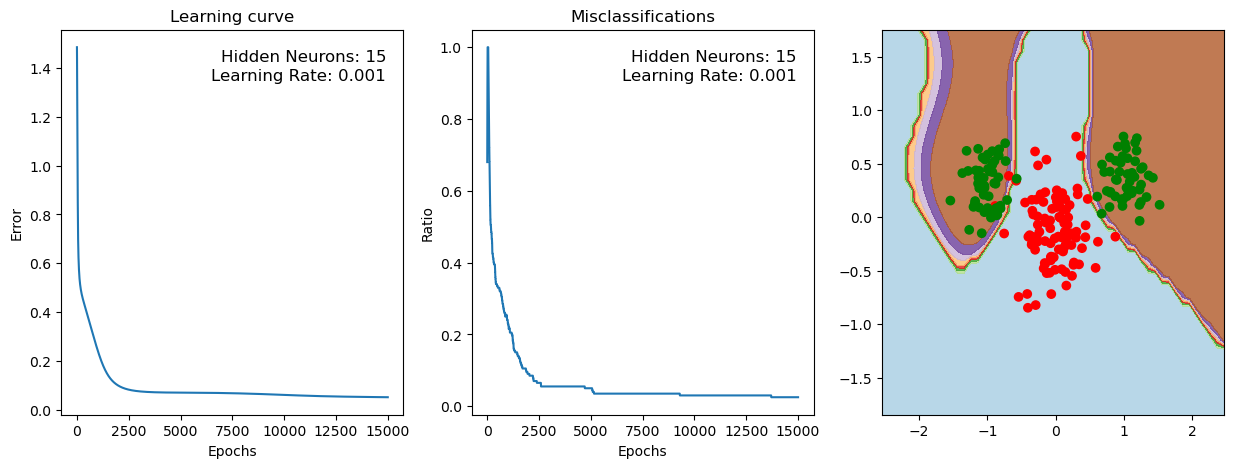
\includegraphics[width=10cm]{Labs/Lab 1/Lab 1b/Figure/15HiddenLayer.png}
    \caption{Results of 15 hidden neurons}
    \label{fig:15Hidden}
\end{figure}
\textbf{Generalization check:}
In this check we generated three scenarios. In the first one we subsample 25\% from each class randomly and train while the rest is for validation. In the second one we subsample 50\% for training and the rest for validation. In the third one we subsample 20\% from a subset of class A which is less than 1 and 80\% from a subset of a class where. class A is more than 0. \\
\\ What was discovered was that that was a overall low generalization error for scenario 1 and 2 if the hidden nodes were more than 1. A generalization error was noticed on most of the networks on scenario 3 however surprisingly they converged. The speed of their convergence had to do with how many hidden nodes there were. They were all trained with a learning rate of 0.0005 as and epochs of 15000 as these numbers allowed us to see the differences in their convergence more easier. Figure \ref{fig: 5 hidden 3 scenarios} is with 5 hidden neurons and Figure \ref{fig: 30 hidden 3 scenarios} is with 30 hidden neurons. The decision bound is drawn on the entire dataset. 
\begin{figure}[!htb]
    \centering
    \begin{subfigure}[b]{0.48\textwidth}
        \centering
        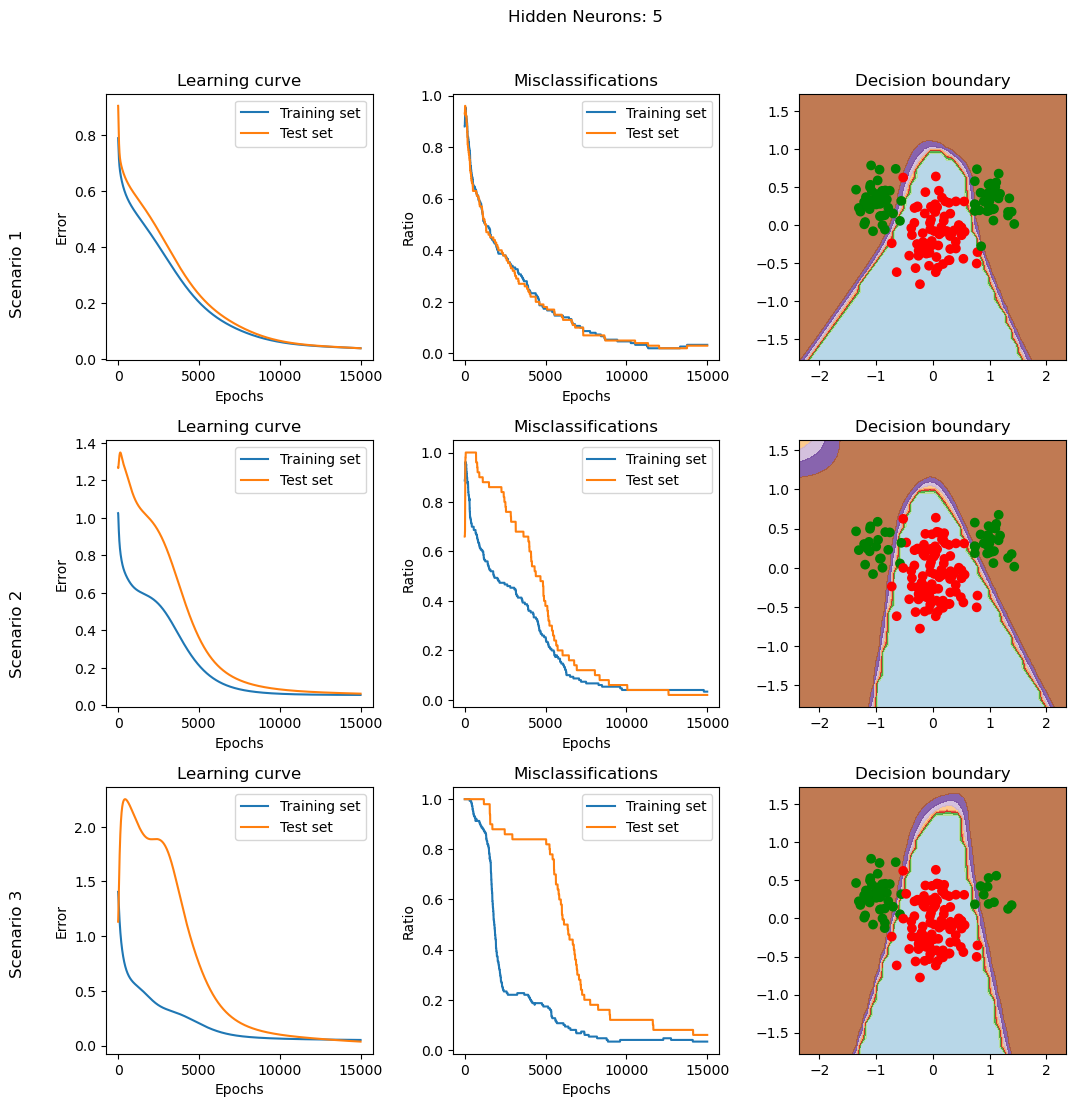
\includegraphics[width=\textwidth]{Labs/Lab 1/Lab 1b/Figure/3.1.1_5 hidden nodes.png}
        \caption{5 Hidden neurons for each scenario}
        \label{fig: 5 hidden 3 scenarios}
    \end{subfigure}%
    \hfill
    \begin{subfigure}[b]{0.48\textwidth}
        \centering
        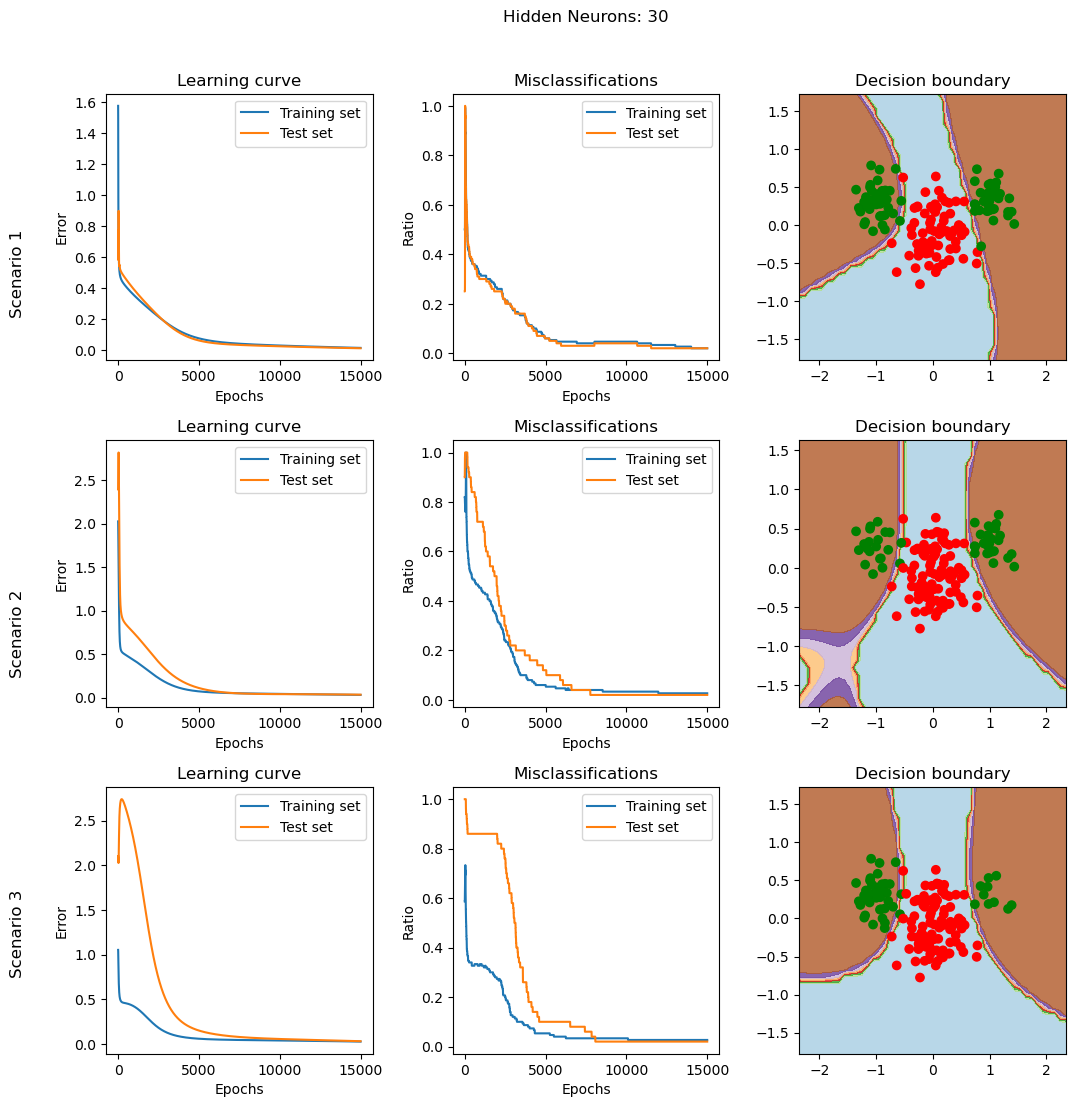
\includegraphics[width=\textwidth]{Labs/Lab 1/Lab 1b/Figure/3.1.1_30 hidden nodes.png}
        \caption{30 Hidden Neurons for each scenario}
        \label{fig: 30 hidden 3 scenarios}
    \end{subfigure}
    \caption{Comparative scenarios with different numbers of hidden neurons}
    \label{fig: comparative scenarios}
\end{figure}\\
\textbf{Regarding Sequential versus batch Learning}: We didn't notice much of a difference in terms in convergence other than sequential made "more changes" per epoch than batch learning. That figure has been purposefully omitted in order to stay within the 8 page limit.\\
\\\textbf{Function approximation of a Gaussian function:} In this part of the assignment we performed regression where we tried to approximate a Gaussian function. 
$$
f(x, y) = e^{-(x^2+y^2)/10} - 0.5
$$
The function can be plotted in three dimensional space where the x and y axis represent the inputs and the z-axis represents the output of the function. The function can be seen in figure \ref{fig:gauss-function} and was plotted with mathplot function in Python.

%% Test
\begin{minipage}{0.5\textwidth}
    \centering
    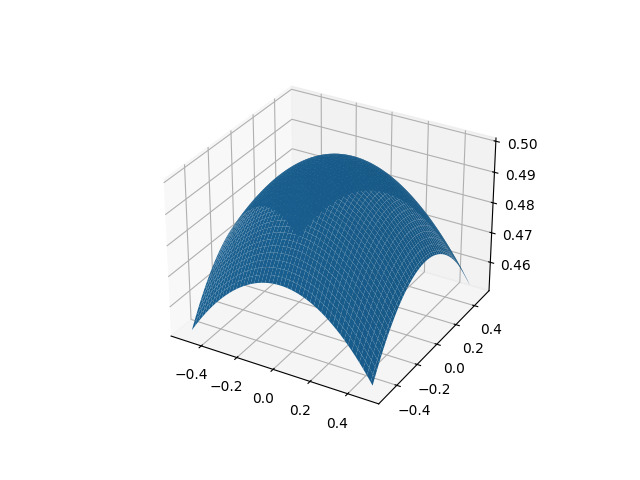
\includegraphics[width=\linewidth]{Labs/Lab 1/Lab 1b/Figure/Figure_1.png}
    \captionof{figure}{The bell shaped gauss function}
    \label{fig:gauss-function}
\end{minipage}%
\hfill% Adds horizontal space between the figure and table
\begin{minipage}{0.45\textwidth}
    \centering
    \captionof{table}{Mean square errors as function of hidden neurons}
    \begin{tabular}{|c|c|}
        \hline
        \# of hidden neurons & Mean square error \\
        \hline
        1 & 0.0001086\\
        \hline 
        4 & $5.96127*10^{-7}$\\
        \hline
        7 & $1.06032*10^{-5}$\\
        \hline
        10 & $2.01543*10^{-5}$\\
        \hline
        13 & $1.85068*10^{-6}$\\
        \hline
        16 & $1.78984*10^{-5}$\\
        \hline
        19 & $4.57150*10^{-5}$\\
        \hline
        22 & $1.49880*10^{-5}$\\
        \hline
        25 & $1.030499*10^{-5}$\\
        \hline
    \end{tabular}
    \label{table:mse}
\end{minipage}

%%
%\begin{figure}[htbp]
%    \centering
%    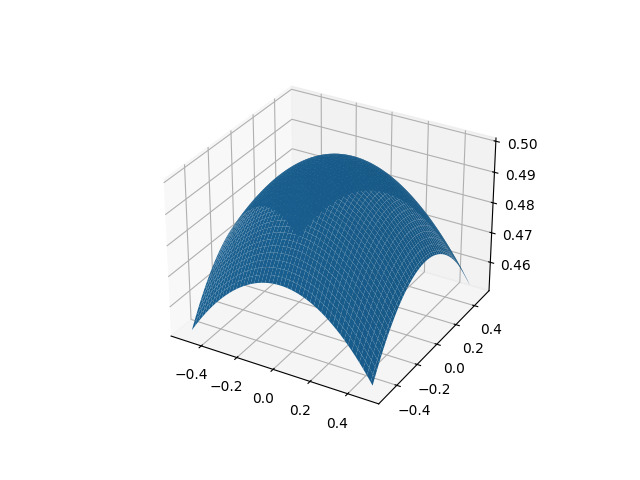
\includegraphics[width=0.5\textwidth]{Labs/Lab 1/Lab 1b/Figure/Figure_1.png}
%    \caption{The bell shaped gauss function}
%    \label{fig:gauss-function}
%\end{figure}

We created a dataset by creating a mesh of x and y values in the interval -0.5 to 0.5. We used 80\% of the dataset as training data and then tested the model using the whole dataset. We varied the number of neurons in the hidden layer from 1-25 with a step size of 3, that is we used a model containing 1, 4, 7 all the way up to 25 neurons in the hidden layer. When training the network we used batch gradient descent with momentum and trained all of the networks for 10000 epochs. We used mean square error as the loss function. The mean square error for each of these models can be seen in table \ref{table:mse}:

%\begin{table}
%\begin{center}
   % \caption{Mean square errors as function of hidden neurons}
  %  \begin{tabular}{|c|c|}

        %\hline
         %\# of hidden neurons & Mean square error \\
        % \hline
       %  1 & 0.0001086\\
     %    \hline 
 %        4 & $5.96127*10^{-7}$\\
  %       \hline
         %7 & $1.06032*10^{-5}$\\
        % \hline
       %  10 & $2.01543*10^{-5}$\\
      %   \hline
     %    13 & $1.85068*10^{-6}$\\
    %     \hline
   %      16 & $1.78984*10^{-5}$\\
         %\hline
         %19 & $4.57150*10^{-5}$\\
        % \hline
       %  22 & $1.49880*10^{-5}$\\
      %   \hline
     %    25 & $1.030499*10^{-5}$\\
    %     \hline
   % \end{tabular}
  %  \label{table:mse}
 %   \end{center}
%\end{table}

As can be seen in Table \ref{table:mse} the mean square error is the lowest when the number of hidden neurons are 4. This is somewhat surprising since a model with more hidden neurons should be able to fit the training data better. One reason for this might be overfitting. The model with only 1 neuron definitely did the worst job at approximating the function. This was expected since the model with one hidden neuron is the one that is the least expressive. A picture of the approximated functions for a few of the models, compared to the true function can be seen in figure \ref{fig:different-hidden-neurons}

\begin{figure}[ht]
    \centering
    \begin{subfigure}{0.4\textwidth}
        \centering
        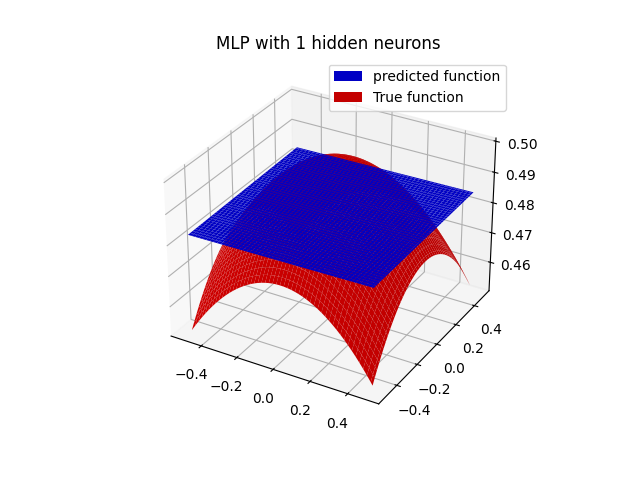
\includegraphics[width=\textwidth]{Labs/Lab 1/Lab 1b/Figure/plots-1-hidden-neurons.png}
        \caption{1 hidden neuron}
    \end{subfigure}
    \hfill
    \begin{subfigure}{0.4\textwidth}
        \centering
        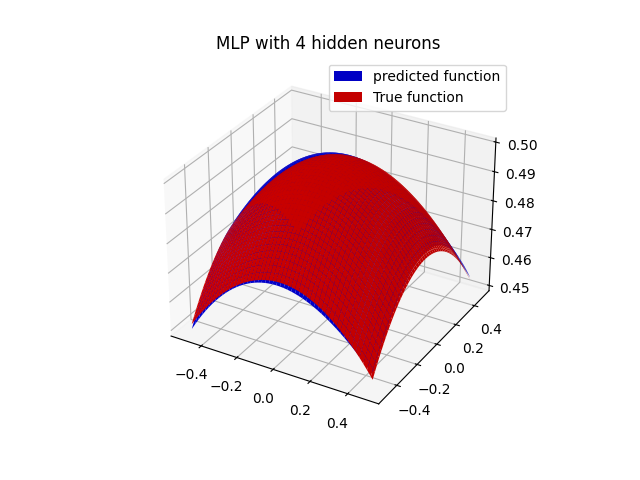
\includegraphics[width=\textwidth]{Labs/Lab 1/Lab 1b/Figure/plots-4-hidden-neurons.png}
        \caption{4 hidden neurons}
    \end{subfigure}
    \begin{subfigure}{0.4\textwidth}
        \centering
        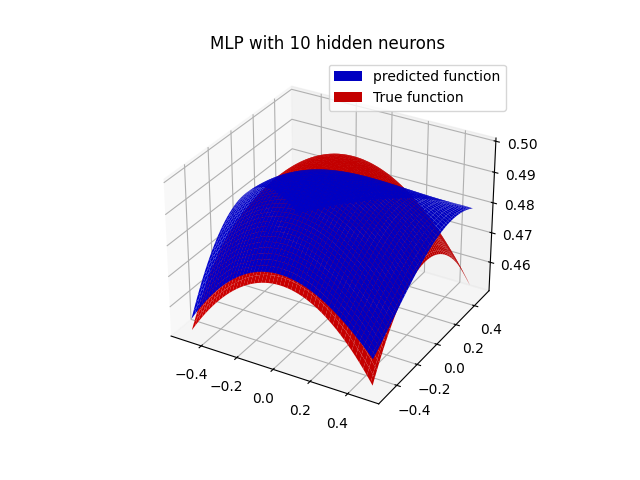
\includegraphics[width=\textwidth]{Labs/Lab 1/Lab 1b/Figure/plots-10-hidden-neurons.png}
        \caption{10 hidden neurons}
    \end{subfigure}
    \hfill
    \begin{subfigure}{0.4\textwidth}
        \centering
        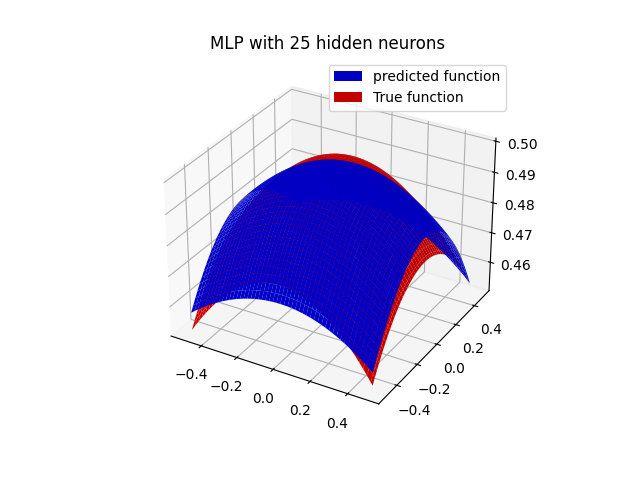
\includegraphics[width=\textwidth]{Labs/Lab 1/Lab 1b/Figure/plots-25-hidden-neurons.png}
        \caption{25 hidden neurons}
    \end{subfigure}
    \caption{Approximation with different amount of hidden neurons}
    \label{fig:different-hidden-neurons}
\end{figure}

We picked the model with 4 hidden neurons as the best model, since it gave us the lowest mean squared error. We then varied the size of the training data. That is we used only a subset of the data for training but we used the whole data set to test the data. We varied the amount of training data from 80\% of the whole data set down to 20\% of the whole data set, with a step size of  10\%. The results for the mean square error was calculated using the whole data set. The results can be seen in table \ref{table:mse-training-data}

\begin{table}
\begin{center}
    \begin{tabular}{|c|c|}
        \hline
         \% of data set used as training data & Mean square error \\
         \hline
         80\% & $1.3094*10^{-7}$\\
         \hline 
         70\% & $1.7549*10^{-6}$\\
         \hline
         60\% & $3.8755*10^{-6}$\\
         \hline
         50\% & $2.9589*10^{-5}$\\
         \hline
         40\% & $7.9677*10^{-6}$\\
         \hline
         30\% & $1.6565*10^{-5}$\\
         \hline
         20\% & $5.0681*10^{-5}$\\
         \hline
    \end{tabular}
    \caption{Mean square errors as function of training data size when using 4 neurons}
    \label{table:mse-training-data}
    \end{center}
\end{table}

As can be seen from the results in table \ref{table:mse-training-data} the mean square error does increase when the amount of training data is decreased. Still the test error is very low when the network is trained using only 20\% of the data. So it seems to generalise pretty well. One reason for that might be that the dataset is very big. That of course helps with generalization. A picture of two of the cases can be seen in figure \ref{fig:generalisation-regression}

\begin{figure}[ht]
    \centering
    \begin{subfigure}{0.4\textwidth}
        \centering
        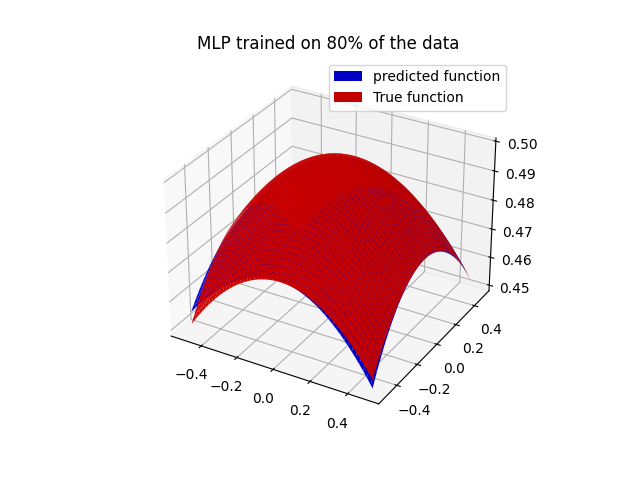
\includegraphics[width=\textwidth]{Labs/Lab 1/Lab 1b/Figure/plots-0.8-train-data.png}
        \caption{80\% of data set}
    \end{subfigure}
    \hfill
    \begin{subfigure}{0.4\textwidth}
        \centering
        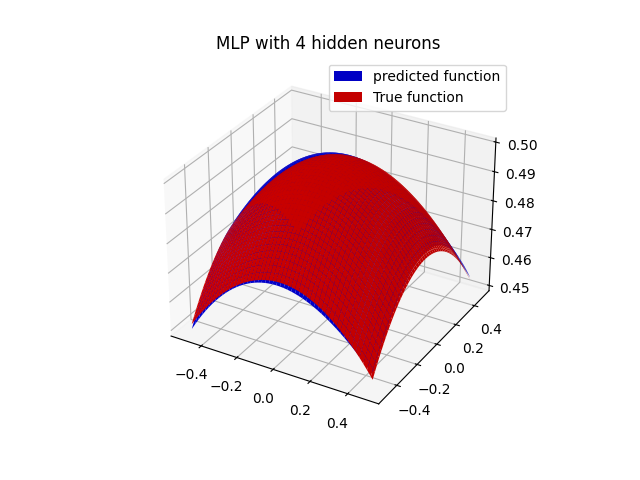
\includegraphics[width=\textwidth]{Labs/Lab 1/Lab 1b/Figure/plots-4-hidden-neurons.png}
        \caption{20\% of data set}
    \end{subfigure}
    \caption{Approximations with varying amount of training data}
    \label{fig:generalisation-regression}
\end{figure}

\subsection{Multi-layer perceptron for time series prediction }
In this section several 2 layered MLP networks were configured for time series forecasting, specifically Mackey-Glass time series. The dataset was broken down into three parts; 800 points for training, 200 for validation and 200 for testing. The testing dataset was used to measure the performance for prediction on unseen data between the best and worst model. The validation dataset was used for model selection. An illustration of how the data was broken down can be seen in figure \ref{fig:Mackey_glass_dataset}.
\begin{figure}[htbp]
    \centering
    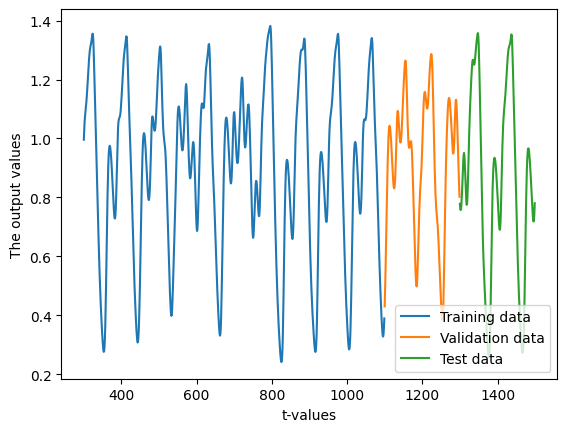
\includegraphics[width=0.5\textwidth]{Labs/Lab 1/Lab 1b/Part2/figure/data.png}
    \caption{The Mackey Glass time series dataset }
    \label{fig:Mackey_glass_dataset}
\end{figure}\\
\\The same result was not replicated after each run therefore each network was ran ten times and the average loss of the runs were taken. Based on the average loss, we could determine which architecture performed the best with respect to the loss. Based on our observations, the lowest loss was obtained when the first layer contained 5 neurons and the second layer with 4 neurons. The largest loss values based on our observations was when the first layer had 3 neurons and the second one with 2 neurons. Their predictions from Mackey Glass time series for t-values between 1300 till 1500 can be seen in figure \ref{fig:Prediction_results_Mackey_glasskit}. As expected, the network which performed the best in the training and validation set also performed the best in prediction/test dataset. The difference between the best performing and the worst performing can be seen in figure \ref{fig:best_loss_comparision}

\begin{figure}[htbp]
    \centering
    \begin{subfigure}[b]{0.45\textwidth}
        \centering
        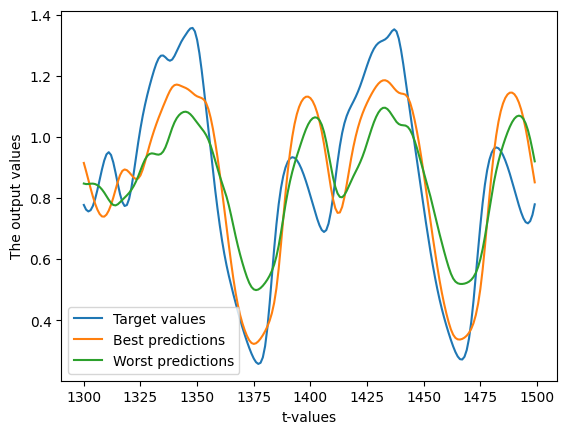
\includegraphics[width=\textwidth]{Labs/Lab 1/Lab 1b/Part2/figure/best_worst_pred.png}
        \caption{Prediction of t-values from 1300 to 1500}
        \label{fig:Prediction_results_Mackey_glasskit}
    \end{subfigure}
    \hfill % This adds a little horizontal space between the subfigures
    \begin{subfigure}[b]{0.45\textwidth}
        \centering
        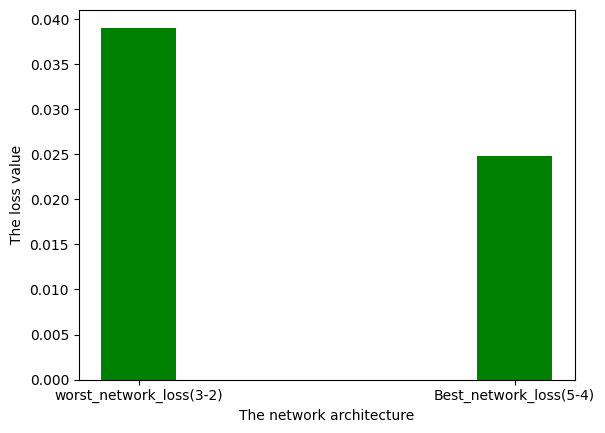
\includegraphics[width=\textwidth]{Labs/Lab 1/Lab 1b/Part2/figure/best_vs_worst_loss.png}
        \caption{The loss of the best and worst network during testing}
        \label{fig:best_loss_comparision}
    \end{subfigure}
    \caption{Comparative Analysis of Network Performances}
    \label{fig:combined_figure}
\end{figure}
\subsubsection{Three-layer perceptron for noisy time series prediction with penalty regularisation}
In this part, we removed the early stopping and started applying the weight decay as a regularization approach. The design was made so that the first hidden layer always consists of 5 nodes, while the number of nodes in the second hidden layer is 3, 6, and $9^6$ neurons respectively as in the instructions. In addition, we added Gaussian noise with zero mean and with 0.05 and 0.15 standard deviance value to the dataset. We did the observation of the three networks based on the validation data as required in the assignment. Then, we measured the performance with four different weight decay constants and with two different standard deviations. We also plotted the training error to see how it is affected in a different architecture. The results can be seen in figure \ref{fig:different-hidden-neurons}

In the design with second hidden layers with many nodes, we noticed the loss of both the training and validation set was constant; it did not change when we changed the regularization constant. The same pattern was in the two values of the standard deviation.

In the design with three nodes, we see that the validation error decreased when we increased the regularization constant with the noise at 0.05. However, we see the opposite pattern when the noise is 0.15, the error increases when we increase the constant. In the network with six nodes, we see that the error decreases in both cases.

\begin{figure}[ht]
    \centering
    \begin{subfigure}{0.4\textwidth}
        \centering
        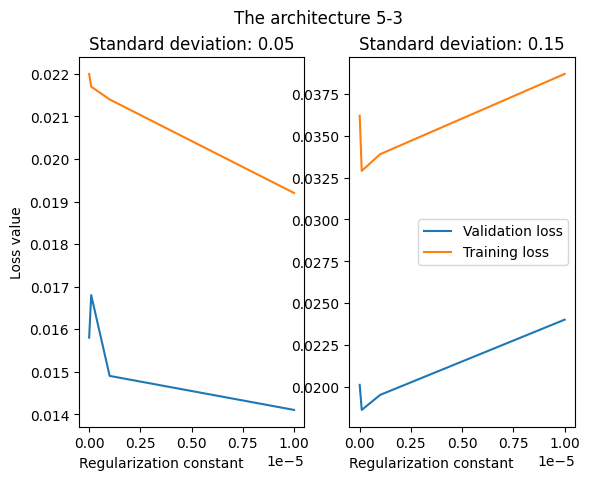
\includegraphics[width=\textwidth]{Labs/Lab 1/Lab 1b/Part2/figure/5-3.png}
        \caption{3 nodes}
    \end{subfigure}
    \hfill
    \begin{subfigure}{0.4\textwidth}
        \centering
        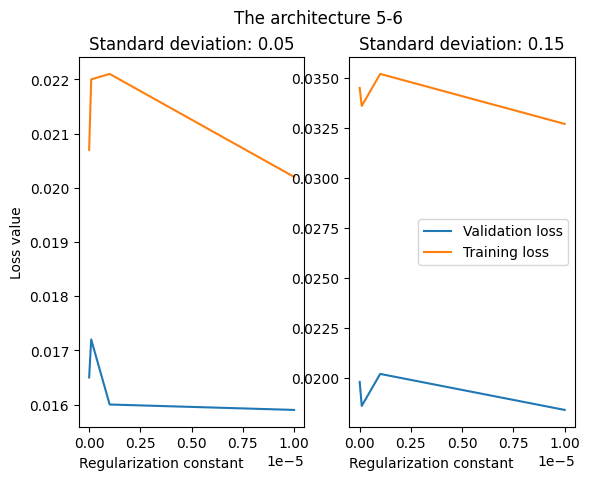
\includegraphics[width=\textwidth]{Labs/Lab 1/Lab 1b/Part2/figure/5-6.png}
        \caption{6 nodes}
    \end{subfigure}
    \begin{subfigure}{0.4\textwidth}
        \centering
        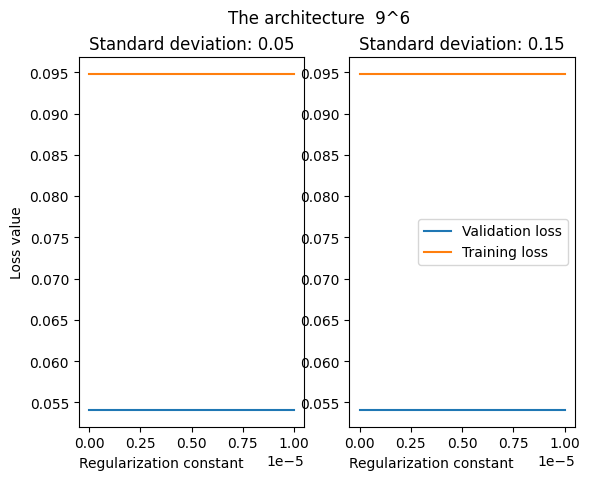
\includegraphics[width=\textwidth]{Labs/Lab 1/Lab 1b/Part2/figure/5-9.png}
        \caption{531441 nodes}
    \end{subfigure}
    \hfill
    \caption{The training and validation error}
    \label{fig:different-hidden-neurons}
\end{figure}

\section{Final remarks }
In this lab we implemented the theoretical concepts from the lectures practically. Several Two-and-three- leveled Multilayered Perceptrons were created and trained using the back propagation algorithm. We learned that:
\begin{itemize}
    \item The amount of hidden neurons in the hidden layers matter however one cannot assume that more neurons means a better generalisation. The appropriate amount of hidden neurons in the hidden layer/s is dependent on the dataset.
    \item Unlike Perceptron learning rule, generalized delta rule with multiple neurons are able to handle linearly non-separable data quite well. 
\item Multilayered perceptrons in our observation are good at approximating functions. When approximating the Gaussian function, most of the architectures approximated the function well.
    \item Multilayered Perceptrons are able to handle time-series forecasting and could be used for it. Relatively simple models which did not take much time to build on our local computers produced decent results when predicting Mackey-Glass series.
    \item Weight initialization matters. The architectures performance is somewhat stochastic depending on the initialization and this affects the time to converge to a final solution and how well the model performs. This is needs to be taken into consideration when building and testing the model.
\item When using weight decay regularisation it generally forces the weights to be smaller and helps with generalisation.
\end{itemize}
\end{document}
